\section{Evaluation}
\label{sec:eval}

\subsection{Experiment 1:  Study of the effect of garbage collection on Spark runtime}
\paragraph{}
Our first set of experiments were conducted to understand the effect of memory pressure on applications by quantifying the impact of garbage collection on a page ranking application written in Spark. The higher level questions that we wanted to answer are as follows:
\begin{enumerate}
\item What is a good strategy of scaling Big data applications ? (more cores, lesser memory per core versus lesser cores, more memory per core) 
\item What is the impact of managed runtimes on application throughput ?
\item Is there a more fundamental problem with the way memory is managed by runtime engines ?
\end{enumerate}
\paragraph{Experimental Setup:}
   	The experiments were conducted on machines with Intel(R) Xeon(R) running at clock frequency of 2.66GHz, with 4 processor cores, with 16 GB of DRAM size. Each machine runs Linux version 2.6.18 with L1 cache size of 32K.  
\paragraph{Experiment 1:}
We conducted the experiments on 5 different configurations. The configurations were as follows:
\begin{itemize}
\item Configuration 1(15W, 1G): The configuration consists of 15 worker nodes, each with 1 GB of memory.
\item Configuration 2(10W, 1G): The configuration consists of 10 worker nodes, each with 1 GB of memory.
\item Configuration 3(5W, 2G):  The configuration consists of 5 worker nodes, each with 2 GB of memory.
\item Configuration 4(2W, 5G):  The configuration consists of 2 worker nodes, each with 5 GB of memory.
\item Configuration 5(1W, 7.5G):The configuration consists of 1 worker node, each with 7.5 GB of memory.
\end{itemize}
Table \ref{tab:table1} lists out the running times, along with the overheads due to the garbage collector for different configurations.

\begin{table}[h!]
\begin{tabular}{| c | c | c | c |}
\hline
Configuration  & Application Run  &  \% Overhead  \\ 
& Time (in ms) & due to GC \\ \hline
15W, 1G & 428,245  & 33\% \\ \hline
10W, 1G & 414,742 &  30.5\% \\ \hline
5W, 2G & 216,320 & 23\%  \\ \hline
2W, 5G & 152159 & 15.29\% \\ \hline
1W, 7.5G & 164893 & 8.45\% \\ \hline
\end{tabular}
\caption{Comparison of the overhead in throughput due to garbage collection for different configurations}
\label{tab:table1}
\end{table}

\paragraph{}
The application we ran was Vanilla Page Ranking algorithm provided with the Spark library. The dataset that we took describes a network which was collected by crawling Amazon website. It is based on \textit{Customers Who Bought This Item Also Bought} feature of the Amazon website. If a product \textit{i} is frequently co-purchased with product \textit{j}, the graph contains a directed edge from \textit{i} to \textit{j} \cite{leskovec2007dynamics}. It describes a graph of \textit{403394 nodes} with \textit{3387388 nodes}. The data is around \textit{50MB} in size. The page ranking algorithm was run for \textit{10 iterations}. 

\paragraph{Analysis of results:}
Fig. \ref{fig:exp4} shows a relative comparison of the overall throughput from the cluster under different configuration settings. Fig. \ref{fig:exp4_2} shows a relative comparison of the impact of garbage collection on the cluster under different configuration settings. We can observe that garbage collection has a detrimental effect on the  overall running time of the application. For a configuration of 2 nodes with 5 GB of memory per server, the overall running time of the application increased by 16\%, whereas for a setup of 15 workers with 1 GB of memory on each server the overall running time of the application was reduced by 33\%. 

\begin{figure}[!ht]
\caption{Comparison of application throughput for different configurations}
\label{fig:exp4}
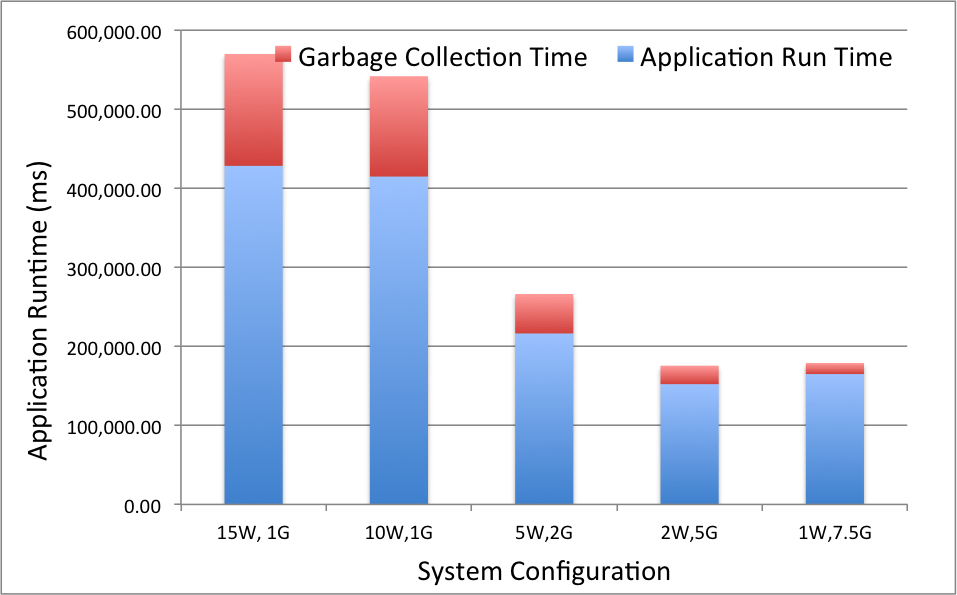
\includegraphics[scale=0.50]{./images/exp4.png}
\end{figure}


\begin{figure}[!ht]
\caption{Comparison of relative affect of garbage collection on application runtime for different configurations}
\label{fig:exp4_2}
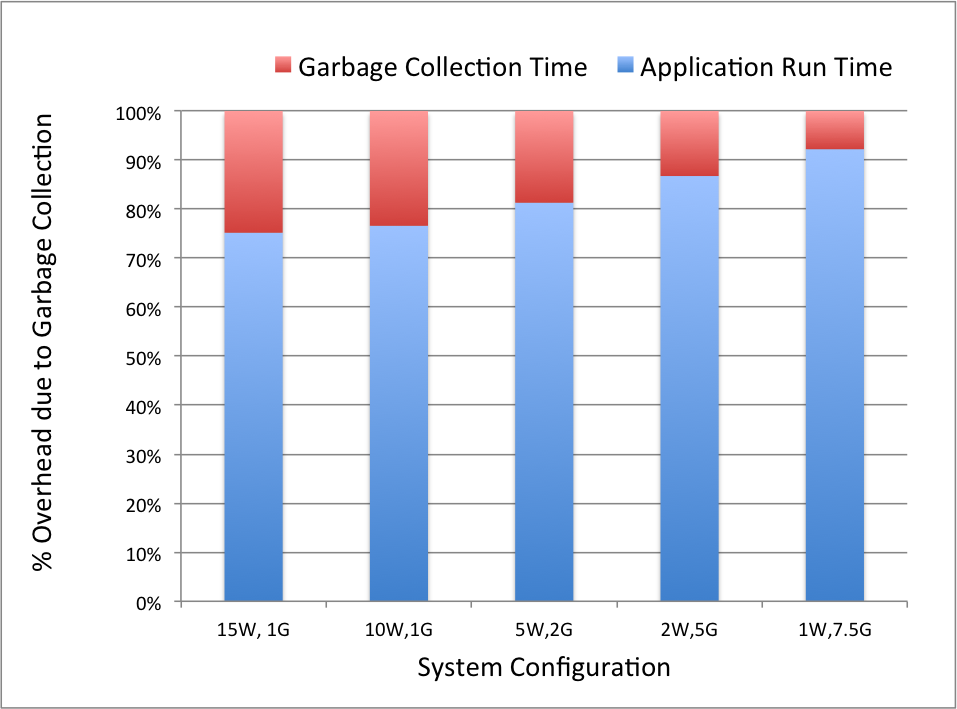
\includegraphics[scale=0.50]{./images/exp4_2.png}
\end{figure}

\begin{figure}[!ht]
\caption{Comparison of application runtime for successive tasks for two different configurations}
\label{fig:exp5}
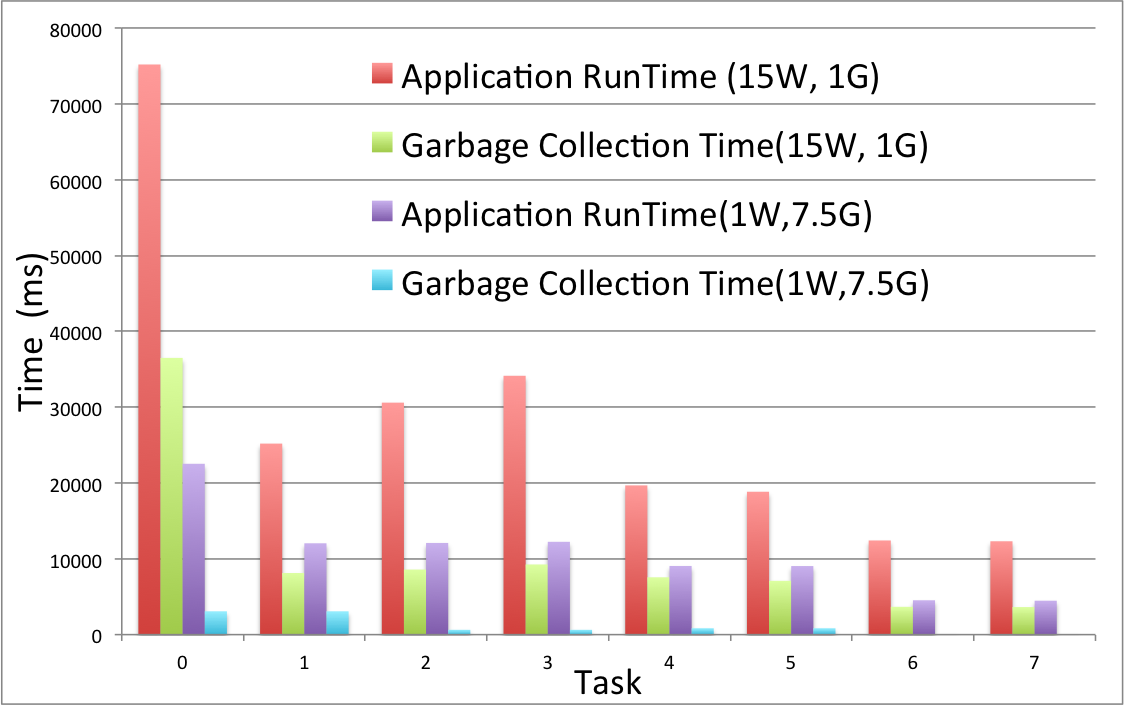
\includegraphics[scale=0.50]{./images/exp5.png}
\end{figure}

\paragraph{}
There are several reasons that explain the above behavior.  Firstly, spark is an in-memory runtime application. It requires extensive amounts of memory for storing intermediate data such as when de-serializing data read from the storage layer, maintaining cache of RDDs, lineages of RDDs etc. Larger memory requirements creates extra memory pressure triggering frequent garbage collection. Therefore the overall throughput of the application decreases. Secondly, in order to scale the application, when the number of nodes in the cluster is increased, the synchronization costs due to communication over the network and secondary storage causes additional overhead.  One of the intuitive conclusions one can derive from the above set of experiments is that in order to scale memory-intensive applications, horizontal scaling may not be as effective as scaling resources on individual nodes. 

\subsection{Experiment 2: Study of object access level patterns within Spark} 
\paragraph{} In order to answer the second question, we took a dummy application in Spark that calculates the value of Pi on a local machine. 
\paragraph{Objective:}
The objective of the experiment was to measure the spectrum of object level accesses when running a baseline spark application that does minimal work. 
\paragraph{Experimental Setup:} 
The experiments were conducted on Intel(R) Xeon(R) CPU E3-1230 V2 machines running at a clock frequency of 3.30GHz with 8 cores with L1 cache size of 32K. For the experiment we used 512MB of memory.
\paragraph{Analysis of results:} 
The results we report are for a specific period of time for which the application runs, since our interception mechanism \ref{sec:design} can approximate object accesses within a single evacuation \cite{fig:exp6} cycle of G1 garbage collection.
Fig. \ref{} shows a histogram based on the object level accesses of different component objects within the spark application. The results indicate a very heavy tailed object level access pattern. Within the specified period, around 45,000 objects were live within the young generation of the application. Out of these, around 1000 objects (nearly 2\%) had an access count of over 1000 per object. We label these objects as hot objects. They account for nearly 58\% of the overall accesses for the given period within the survivor and eden regions. Nearly, 17\% of the overall accesses derive from 0.02\% of the total number of objects. Nearly, 3\% of the overall accesses are for 50\% of the objects in the specified regions of the memory.  These numbers clearly indicate that object access patterns within applications are extremely heavy tailed. 

\begin{figure}[!ht]
\caption{Histogram of object accesses for different objects for a Spark Application}
\label{fig:exp6}
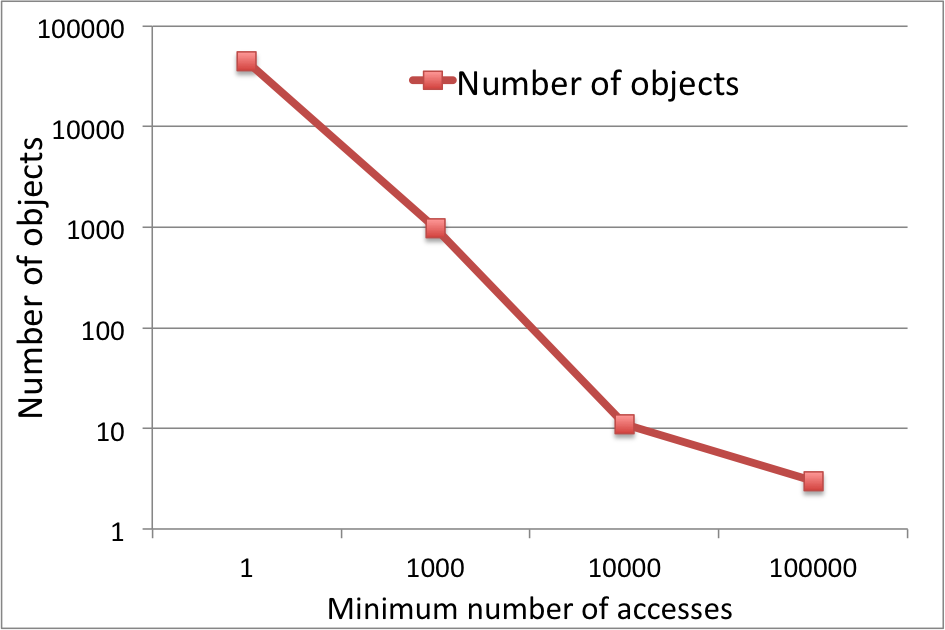
\includegraphics[scale=0.50]{./images/exp6.png}
\end{figure}

\paragraph{}
Most of the data objects that were accessed more frequently were arrays of utility functions such as worker queue, XML document handlers, symbol table entry handlers, loggers etc. The objects that were less frequently accessed were temporary objects such as method objects, strings, classes for caching root names, object for looking up the mime types (used for inspecting header of objects), objects created for storing symbol tables for compilers, parsers etc. There are three reasons explaining the heavy tail in the specific distribution pattern of object level accesses. Firstly, accesses to large arrays of objects (such as RDDs) will have specifically high values since each access of an object within an array is also an access to the array (understood as a container of objects). Such arrays can be considered hotspots within the object space. Secondly, instances of objects that contain utility functions such as compression of data, methods for polling the network interfaces, DOM parsers etc. have large access counts. These objects are accessed more ubiquitously due to their generic functions and therefore are hot in their access patterns. Thirdly, a very large collection of objects (nearly half of all the objects) such as classes for caching root names might get accessed once and be used only at certain specific intervals, such as that at a task start up for looking up the addresses of the different workers.  These "cold" objects show low usage access pattern. 
\paragraph{}	
The intuition that one can develop from this experiment that access patterns within memory intensive workloads (such as those used by Spark) have extremely long tails. Such access patterns unearth a potential problem within contemporary memory management system designs. Current virtual memory systems have a paged based abstraction for managing application data. Our intuition is that data residing on similar pages might not always have very good "access similarity". Paging, therefore, by virtue of its underlying design cannot capture the access level semantics of applications at finer granularity. This experiment provides us with useful insights and helps further our understanding of the underlying fundamental problems within current memory management system designs.

\subsection{Study of indexing within RDDs:}
\paragraph{Objective:} We observe that while the design of RDDs supports caching and faster recovery through lineages, it lacks certain capabilities. Besides, RDDs inherently support operations on data sets which consist of pairs of key and values. We posit a natural extension to the design of RDDs using range partitioned indexes on keys. This experiment answers the following three questions:
\begin{enumerate}
\item Is there more efficient way of running queries on semi-structured data stored in files (database logs, page visit logs) ? 
\item What are better schemes of indexing larger datasets using  RDDs ?
\item How well can a generic indexing scheme based on range partitioning scheme scale ? 
\end{enumerate}
\paragraph{Experimental Setup:} The experiments were conducted on machines with Intel(R) Xeon(R) CPU E3-1230 V2 running at a clock frequency of 3.30GHz, with 8 processor cores, with 32 GB of DRAM size. Each machine runs Linux version 3.11.10 with L1 cache size of 32K.  The experiments were run on a cluster of 3 nodes connected with 1 Gb/s NICs arranged on a single rack. The Spark setup consisted of 6 workers (2 on each machine) and 1 master. Each of the workers was configured with 8GB of memory and the master had 2 GB of memory.  The master was set up on the same machine as one of the workers. The tests were run using using the Spark shell interface.  The experiments were conducted on Hadoop file system. The version of Hadoop was 2.2.0.  The block size was set to default 256MB. The Hadoop master and data node were set up on the same machine.

\paragraph{Benchmarking DataSet:} For the experiments we used page view logs from Wikimedia dumps \cite{wikimedia}. Wikipedia publishes page view statistics every month. The following is an example of the data:  \textit{fr.b Special:Recherche/Achille\_Baraguey\_d\%5C\%27Hilliers 1 624}. In the above example, the first column ("fr.b") denotes the project name. The second column is the title of the page retrieved, the third column is the number of requests, and the fourth column is the size of the content returned.  In our experiments, we use the project name as the key and the rest of the line as the value that needs to be retrieved from the underlying distributed file system.  We use two different collection of data (10 GB, 25 GB) of data, approximating 5 months and 1 years of data respectively, with nearly 300 million and 730 million records. 

\paragraph{Experiment 3:}
For the experiments we run five different queries and measure the overall time it takes for the queries to complete. 
Fig. \ref{fig:exp7} shows a comparison of three different configurations when running the queries on 10GB file. VSpark denotes queries on vanilla spark using unindexed RDDs, ISpark\_C (Indexed Spark Coarse Grained Partitioned) denotes RDDs with 320 partitions and ISpark\_F (Indexed Spark Fine Grained) denotes RDDs with 1280 partitions. While VSpark takes 87 seconds to complete , the average time for a positive query (a query that matched keys in the file) was around 37 seconds. Using, more fine grained partitioning, the average time to 11 seconds. Another interesting observation to note is that for queries that miss, the result is returned in under a second. The underlying reason for the improvement in performance is that the range partitioning mechanism can pre-determine the set of RDDs on which the query needs to be run. This, reduces the overall computation that needs to done for filtering records. Besides, the communication cost over the network is reduced. This results in good enhancement in the performance. For queries, that result in a miss, the master can instantaneously return a null result, since it can ensure that key is outside the range of all the partitions.

\begin{figure}[!ht]
\caption{Comparison of query completion times between Spark, Spark-Coarse grained and Spark-Fine grained partitioned for a 10 GB file}
\label{fig:exp7}
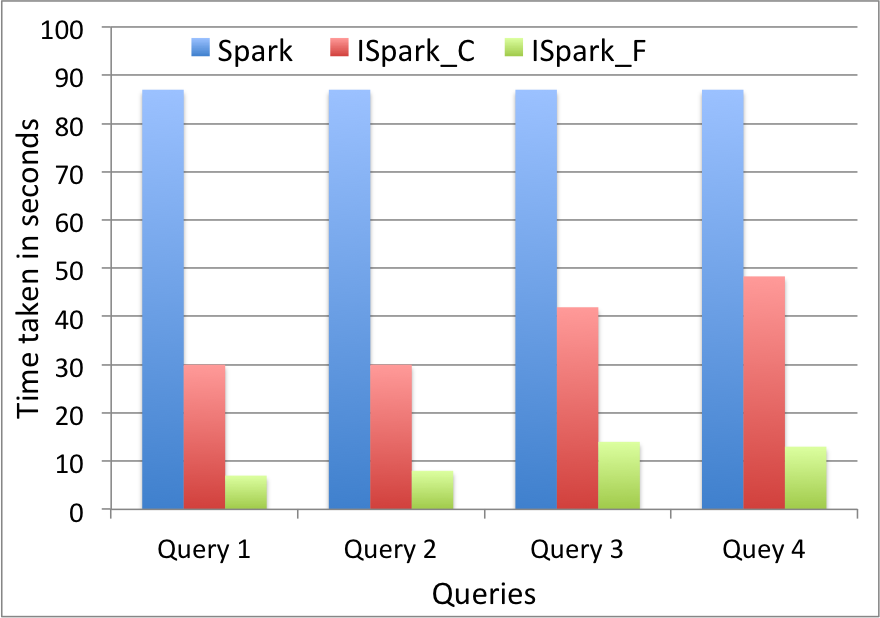
\includegraphics[scale=0.50]{./images/exp7.png}
\end{figure}

\paragraph{}
Fig. \ref{fig:exp8} shows a comparison of three different configurations when running the queries on 25 GB file. The number of partitions for ISpark\_C were 1572 and that for ISpark\_F were 10000. While VSpark takes 220 seconds to complete , the average time for a positive query (a query that matched keys in the file) was around 49 seconds. Using, more fine grained partitioning, the average time to 9 seconds. We can observe, that while VSpark scales poorly as the size of the data increases, indexes helps the filtering query to scale in a more scalable manner. With more fine grained partitioning, we were able to reduce the overall query time for a 25GB over 10GB. However, we cannot increase the number of partitions since the master node would have limited amount of memory. In order to scale up, we can maintain a separate indexing server that can cache indexes and return the set of RDDs on which a query has to be run. 

\begin{figure}[!ht]
\caption{Comparison of query completion times between Spark, Spark-Coarse grained and Spark-Fine grained partitioned for a 25 GB file}
\label{fig:exp8}
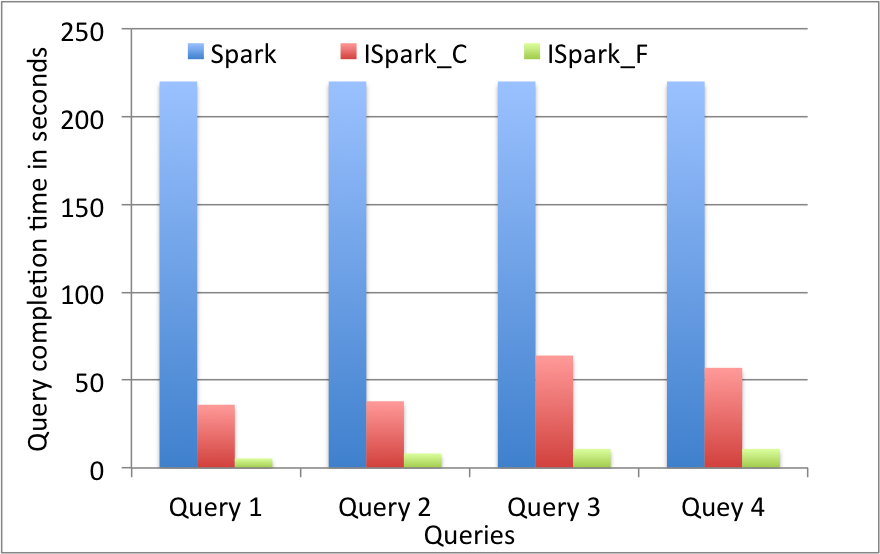
\includegraphics[scale=0.50]{./images/exp8.png}
\end{figure}

\paragraph{}
Fig. \ref{fig:exp9} shows the overall time it takes for the indexing mechanism to set up the partitions on the range of RDDs. The partitioning scheming scales in accordance with the filtering mechanism since the all the set of records have to be filtered. However, since, this is a one time cost, the cost can be amortized with a batch of queries. Besides, as the number of partitions increases, the time it takes to build an index does not increase by a large amount. Therefore, fine grained indexing can be very useful as long the master has sufficient memory to hold the index.

\begin{figure}[!ht]
\caption{Comparison of index creation time}
\label{fig:exp9}
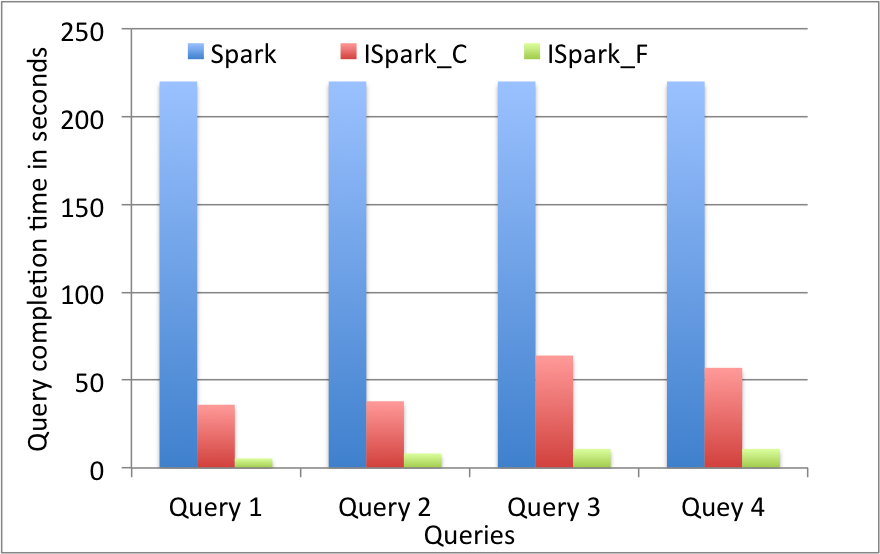
\includegraphics[scale=0.50]{./images/exp8.png}
\end{figure}
